% =====================================================================
%  Esboço de artigo - Macroeconomia e Finanças (Prof. Helder Ferreira de Mendonça)
%  Compilar no Overleaf com pdfLaTeX. Trechos em cinza [assim] são números a atualizar
%  depois de rodar 05_helder.R e 06_capitais_helder.R (pasta Documentos > helder).
% =====================================================================
\documentclass[12pt,a4paper]{article}

\usepackage[utf8]{inputenc}
\usepackage[T1]{fontenc}
\usepackage[brazil]{babel}
\addto\captionsbrazil{\renewcommand{\tablename}{Tabela}}
\usepackage{mathptmx}
\usepackage{amsmath}
\usepackage[top=2.5cm, left=2.5cm, bottom=2.5cm, right=2.5cm]{geometry}
\usepackage{setspace}
\onehalfspacing
\usepackage{indentfirst}
\setlength{\parindent}{1.25cm}
\usepackage{microtype}
\usepackage{booktabs}
\usepackage{tabularx}
\usepackage{float}
\usepackage{graphicx}
\usepackage{threeparttable}
\usepackage[hidelinks]{hyperref}
\usepackage{xcolor}
\newcolumntype{L}{>{\raggedright\arraybackslash}X}
\newcommand{\afazer}[1]{\textcolor{gray}{[#1]}}

\title{\bfseries Choque regional temporário e mercado de trabalho:\\
efeitos locais e de transbordamento da COP30 sobre o emprego formal no Pará}
\author{Marcela Paz da Silva Enriquez\\[2pt]
\small PPGE/UFF -- Macroeconomia e Finanças\\
\small Versão revisada para discussão}
\date{Novembro de 2026}

\begin{document}
\maketitle

\begin{abstract}
\noindent Grandes eventos são justificados pela promessa de gerar empregos, mas a evidência
\textit{ex post} sugere efeitos pequenos e passageiros. Este artigo trata a COP30, realizada em
Belém em novembro de 2025, como um choque de demanda regional, temporário e anunciado com
antecedência, e investiga se ele alterou o emprego formal em Alojamento e Alimentação na cidade-sede,
se transbordou para os municípios vizinhos e se apareceu também nos preços locais. Com microdados do
Novo CAGED por município e mês (jan/2022--jul/2026) e o IPCA da Região Metropolitana de Belém,
estimam-se três modelos por mínimos quadrados ordinários: (A) séries por grupo de municípios, com
sazonalidade, tendência e controles macroeconômicos nacionais, com erros de Newey-West; (B) um painel
de municípios com efeitos fixos (diferenças em diferenças), que separa efeito local e transbordamento,
tendo o interior do estado como comparação; e (C) a inflação de hospedagem e de alimentação fora do
domicílio em Belém relativa à do Brasil. Os resultados apontam um choque local, temporário e
concentrado na hospedagem: o emprego no Alojamento de Belém sobe na preparação e no evento e recua
na desmobilização, sem transbordamento positivo para os vizinhos e sem ganho líquido para a região.
Como há uma única cidade tratada, a inferência é feita por placebo, e a evidência é mais forte para
o Alojamento do que para o setor agregado. \afazer{Acrescentar uma frase com o resultado de preços
(Modelo C) e com a comparação com as capitais.}

\medskip\noindent\textbf{Palavras-chave:} megaeventos; choques regionais; mercado de trabalho;
inflação regional; COP30.\quad \textbf{JEL:} R11, J21, E31, Z32.
\end{abstract}

% ---------------------------------------------------------------------
\section{Introdução}

Governos costumam justificar grandes eventos pela geração de empregos. A COP30, a primeira
conferência do clima da ONU realizada na Amazônia, não foi exceção: entre o anúncio, em 2023, e a
realização, em novembro de 2025, Belém recebeu investimentos em infraestrutura, hospedagem e
serviços, e uma demanda concentrada de visitantes durante duas semanas. Do ponto de vista
macroeconômico, trata-se de um \textbf{choque de demanda regional}: concentrado no espaço (uma região
metropolitana), no tempo (um mês) e em poucos setores (hospedagem e alimentação), e anunciado com
antecedência, o que permite separar antecipação, impacto e dissipação.

Um choque de demanda regional pode ser absorvido por quantidades (mais emprego), por preços (diárias
e refeições mais caras) ou por deslocamento de trabalhadores entre localidades (Blanchard e Katz,
1992). O artigo investiga os três canais, com uma pergunta central: \textbf{o emprego gerado pela
COP30 ficou em Belém, espalhou-se pelos municípios vizinhos ou foi apenas realocado dentro da
região, e o choque apareceu também nos preços?} A resposta importa para a avaliação de megaeventos
como política de desenvolvimento regional: se o emprego apenas migra de um município para outro, ou se
o choque se dissipa em preços, o ganho agregado de emprego na região é pequeno, mesmo que a cidade-sede
registre aumento.

\textbf{Inspiração do desenho.} A estratégia empírica combina três referências. A separação do efeito
em cidade-sede, vizinhos e região é inspirada em \textit{Big Plants in Small Towns: Labor
Concentration and Land Use in Rural Brazil} (Di Pietra et al., 2026), trabalho aceito no 48º Encontro
Brasileiro de Econometria, que mede o efeito de um grande empregador sobre o emprego formal na cidade
que o recebe (+10,8\%), nos vizinhos ($-1{,}9\%$) e na microrregião (+1,45\%). O tratamento de uma
única unidade atingida, com um grupo vizinho ``potencialmente tratado'' e efeitos separados para
``durante'' e ``depois'', segue Leoni e Boto-García (2023), publicado na \textit{Environmental and
Resource Economics}, sobre a erupção vulcânica de La Palma. A especificação em séries mensais com
dummies de sazonalidade e do evento segue a literatura de megaeventos publicada em periódicos, em
especial Baumann e Matheson (2018) e Hagn e Maennig (2009). O componente macroeconômico, por fim,
dialoga com Mendes Garcia e Mendonça (2026), que mostram que choques de origem climática têm efeitos
inflacionários desiguais entre as regiões brasileiras.

\textbf{Contribuição.} (i) Avaliação \textit{ex post} de uma conferência do clima sobre o mercado de
trabalho, com dados administrativos mensais, tema pouco explorado pela literatura de megaeventos, que
se concentra em eventos esportivos; (ii) decomposição do efeito em local, de transbordamento e
regional; (iii) teste conjunto dos canais de quantidade (emprego) e de preço (inflação local); e
(iv) separação entre o choque do evento e o ciclo macroeconômico nacional.

% ---------------------------------------------------------------------
\section{Literatura e mecanismo}

\textbf{Megaeventos e emprego.} A literatura encontra efeitos modestos, concentrados no turismo e no
período do evento: Copa do Mundo de 2006 na Alemanha (Hagn e Maennig, 2009), Jogos Olímpicos de
Atlanta em 1996 (Feddersen e Maennig, 2013), Copa do Mundo de 2014 no Brasil (Baumann e Matheson,
2018) e Jubileu de 2000 em Roma (Bronzini, Mocetti e Mongardini, 2019).

\textbf{Ajuste regional a choques de demanda.} Em Blanchard e Katz (1992), um choque de demanda
regional se ajusta por três margens: emprego local, salários e preços, e migração de trabalhadores
entre regiões. Moretti (2010) acrescenta que um choque em um setor pode gerar empregos em outros
setores da mesma cidade (multiplicador local). Desse arcabouço decorrem as previsões do artigo:
\begin{enumerate}\itemsep0pt
\item \textbf{Quantidade:} o emprego em Belém aumenta na preparação e no evento e recua depois, com
efeito maior na hospedagem, setor mais exposto à demanda de visitantes;
\item \textbf{Transbordamento:} o emprego dos vizinhos pode subir (multiplicador e fornecedores) ou
cair (deslocamento de trabalhadores para a sede);
\item \textbf{Preço:} se a oferta de quartos e refeições é pouco elástica no curto prazo, parte do
choque aparece em preços, e a inflação de hospedagem e de alimentação fora do domicílio em Belém
supera a do Brasil durante o evento.
\end{enumerate}

\textbf{Choques climáticos e inflação regional.} Mendes Garcia e Mendonça (2026) mostram que o mesmo
choque climático tem efeitos inflacionários distintos entre os estados brasileiros, conforme a
estrutura de consumo de cada um. Este artigo examina um choque associado à agenda climática,
espacialmente concentrado, e mede sua incidência tanto em quantidades quanto em preços locais.

% ---------------------------------------------------------------------
\section{Dados}

A base principal é um painel de municípios paraenses por mês, de janeiro de 2022 a julho de 2026
(55 meses), construído a partir de microdados públicos (Tabela~\ref{tab:dados}). O resultado de
interesse é o saldo de empregos formais (admissões menos desligamentos) nas divisões 55 (Alojamento)
e 56 (Alimentação) da CNAE 2.0, normalizado pela média mensal de admissões de cada município no
período de referência (jan/2022--jun/2024):
\begin{equation}
y_{it} = 100 \times \frac{\text{adm}_{it} - \text{desl}_{it}}{\overline{\text{adm}}_{i}^{\,\text{ref}}}.
\end{equation}
Assim, $y_{it} = 10$ significa um saldo equivalente a 10\% de um mês normal de contratações, o que
torna comparáveis municípios de tamanhos muito diferentes. Para a interpretação, os efeitos estimados
são também convertidos em \textbf{vagas por mês}, multiplicando-se o coeficiente pelas admissões
normais do município e dividindo-se por 100. Entram no painel os municípios com média de pelo menos
cinco admissões mensais no setor no período de referência: 31 municípios e 1.705 observações. Os
municípios são divididos em Belém (tratada); demais municípios da Região Metropolitana -- Ananindeua,
Marituba, Benevides, Santa Bárbara do Pará, Santa Izabel do Pará e Castanhal, dos quais cinco passam o
corte (potencialmente tratados); e interior do estado (comparação). Uma segunda base, usada como
robustez, reúne as 26 capitais estaduais (exceto o Rio de Janeiro, sede da Cúpula do G20 em novembro
de 2024), construída da mesma forma.

\begin{table}[H]
\centering\footnotesize
\caption{Variáveis, fontes e extração}\label{tab:dados}
\begin{tabularx}{\linewidth}{p{3.1cm}p{3.3cm}L}
\toprule
\textbf{Variável} & \textbf{Fonte} & \textbf{Extração}\\
\midrule
Admissões, desligamentos e saldo (CNAE 55 e 56), por município e mês &
Novo CAGED, MTE: \url{ftp://ftp.mtps.gov.br/pdet/microdados/NOVO\%20CAGED/} &
Arquivos mensais MOV, FOR e EXC; filtro UF = 15 (ou código das capitais) e subclasse CNAE iniciada em
55 ou 56; saldo = MOV + FOR $-$ EXC, por mês de competência; soma por município (código IBGE de 6
dígitos)\\
\addlinespace
IPCA por item, RM de Belém e Brasil & IBGE/SIDRA, Tabela 7060: \url{https://sidra.ibge.gov.br/tabela/7060} &
Variação mensal (\%) de ``Alimentação fora do domicílio'' e ``Hospedagem''; nível territorial Região
Metropolitana (Belém) e Brasil\\
\addlinespace
Atividade econômica nacional & BCB-SGS, série 24364 (IBC-Br dessazonalizado): \url{https://www3.bcb.gov.br/sgspub} &
Variação percentual mensal\\
\addlinespace
Câmbio R\$/US\$ & BCB-SGS, série 3698 & Dólar comercial, venda, média do mês; variação \% mensal\\
\addlinespace
Selic & BCB-SGS, série 4390 & Taxa acumulada no mês (\% a.m.); variação mensal (p.p.)\\
\addlinespace
IPCA nacional & BCB-SGS, série 433 & Variação mensal (\%)\\
\bottomrule
\end{tabularx}
\end{table}

Duas escolhas sobre os controles merecem destaque. Primeiro, a atividade econômica é medida pelo
IBC-Br \textbf{nacional}, e não pelo volume de serviços do Pará: este último é afetado pela própria
COP30 e seria um controle pós-tratamento, que absorveria parte do efeito que se quer medir. Segundo,
câmbio, atividade e Selic entram em variação, e não em nível, para evitar regressões espúrias entre
séries com tendência (Granger e Newbold, 1974). Toda a extração é feita em R pelos scripts
\texttt{05\_helder.R} e \texttt{06\_capitais\_helder.R}, que baixam os dados das fontes acima e
reproduzem a base do zero.

% ---------------------------------------------------------------------
\section{Estratégia empírica}

O período posterior ao anúncio é dividido em três fases: preparação ($\text{Prep}_t$,
jul/2024--out/2025), evento ($\text{Evento}_t$, nov/2025) e desmobilização ($\text{Desmob}_t$,
dez/2025--jul/2026).

\subsection{Modelo A: séries por grupo e ciclo macroeconômico}

Para cada grupo $g$ (Belém, demais municípios da RM, RM inteira e interior), estima-se por MQO
\begin{equation}
y_{gt} = \beta_P\,\text{Prep}_t + \beta_E\,\text{Evento}_t + \beta_D\,\text{Desmob}_t
       + \sum_{m=2}^{12}\mu_m M_{mt} + \delta t + \gamma' X_t + \varepsilon_{gt},
\end{equation}
em que $M_{mt}$ são dummies de mês do ano (sazonalidade, inclusive o Círio de Nazaré em outubro), $t$
é uma tendência linear e $X_t$ reúne as variações do IBC-Br, do câmbio e da Selic e o IPCA nacional. Os
coeficientes $\beta$ medem o desvio médio do saldo em cada fase em relação ao padrão sazonal, à
tendência e ao ciclo macroeconômico. Como os resíduos de séries mensais tendem a ser
autocorrelacionados, os erros-padrão são de Newey e West (1987). A especificação segue Baumann e
Matheson (2018), que avaliam a Copa do Mundo de 2014 no Brasil com dados mensais, dummies de mês,
controles para o ambiente macroeconômico, dummies para os meses do evento e testes de raiz unitária, e
Hagn e Maennig (2009); a leitura do choque como choque de demanda regional que se ajusta por
emprego, preços e migração segue Blanchard e Katz (1992). Os grupos são formados pela soma dos municípios, de modo que municípios maiores
pesam mais; a coluna ``RM inteira'' indica se o choque gerou emprego líquido na região ou apenas
realocação. O Modelo A não tem grupo de comparação: ele mostra se o padrão observado resiste ao
controle do ciclo macroeconômico, e não identifica, sozinho, o efeito causal.

\subsection{Modelo B: diferenças em diferenças -- efeito local e transbordamento}

A estratégia causal é um modelo de diferenças em diferenças com efeitos fixos, no qual o interior do
estado fornece o contrafactual:
\begin{equation}
y_{it} = \alpha_{i,m(t)} + \lambda_t + \sum_{f} \beta^{\text{Bel}}_f\,(\text{Bel}_i \times F_{ft})
       + \sum_{f} \beta^{\text{RM}}_f\,(\text{RM}_i \times F_{ft}) + \varepsilon_{it},
\end{equation}
em que $F_{ft}$ são as fases, $\text{Bel}_i$ indica Belém e $\text{RM}_i$ indica os demais municípios
da Região Metropolitana. O efeito fixo $\alpha_{i,m(t)}$ (município $\times$ mês do ano) absorve o
nível e a sazonalidade de cada município; o efeito fixo de mês $\lambda_t$ absorve tudo o que atinge o
estado no mesmo mês, inclusive o ciclo macroeconômico, razão pela qual os controles macro não entram
neste modelo. $\beta^{\text{Bel}}$ é o \textbf{efeito local} e $\beta^{\text{RM}}$ é o
\textbf{transbordamento}: positivo indica difusão; negativo, deslocamento de trabalhadores para a sede.
Diferentemente do Modelo A, cada município tem o mesmo peso. O desenho segue a literatura que mede
choques locais comparando a área atingida com áreas semelhantes: Greenstone, Hornbeck e Moretti (2010)
comparam condados que receberam grandes plantas industriais com os que disputaram e perderam a
instalação, e Faber e Gaubert (2019) estimam os efeitos locais e de transbordamento do turismo sobre o
emprego nos municípios do litoral mexicano. A resposta do emprego em setores não comercializáveis,
como hotéis e restaurantes, a choques de demanda local é documentada por Mian e Sufi (2014). A hipótese de identificação é a de
tendências paralelas, avaliada por um estudo de evento que estima um coeficiente para cada mês de 2023
a 2026 (base: 2022): os coeficientes anteriores a julho de 2024 devem ser próximos de zero
(Freyaldenhoven, Hansen e Shapiro, 2019).

\textbf{Inferência.} Com uma única unidade tratada, o erro-padrão agrupado por município não é
confiável para o efeito de Belém (Conley e Taber, 2011). A significância é, por isso, avaliada por
placebo: a estimação é repetida com cada um dos 25 municípios do interior no lugar de Belém, e o
p-valor é a proporção de efeitos, em módulo, maiores ou iguais ao de Belém. Como os municípios do
interior são menores e mais voláteis, cada efeito é também dividido pelo desvio-padrão do saldo do
município no período de referência, à maneira da razão entre erros pós e pré-tratamento do controle
sintético (Abadie, Diamond e Hainmueller, 2010). As estrelas de erro agrupado são reportadas apenas
como referência.

\subsection{Modelo C: canal de preços}

Para verificar se o choque apareceu em preços, estima-se, para cada item $k$ do IPCA (alimentação fora
do domicílio, hospedagem e índice geral),
\begin{equation}
\pi^{\text{Belém}}_{kt} - \pi^{\text{Brasil}}_{kt} = \theta_P\,\text{Prep}_t + \theta_E\,\text{Evento}_t
+ \theta_D\,\text{Desmob}_t + \sum_{m=2}^{12}\mu_m M_{mt} + u_{kt},
\end{equation}
em que $\pi$ é a variação mensal do preço. A diferença em relação ao Brasil retira choques nacionais de
preços, de modo que $\theta_E > 0$ indica inflação local acima da nacional no mês do evento. A
estratégia de comparar a inflação de uma região com a nacional diante de um choque de demanda regional
segue Nakamura e Steinsson (2014), que usam gastos militares nos estados americanos para medir a
resposta regional do produto e dos preços. Os
erros-padrão são de Newey-West.

\subsection{Estacionariedade e escolha do modelo: por que não VAR, VEC ou painel dinâmico}

Estimadores GMM para painéis dinâmicos (Arellano e Bond, 1991) foram desenhados para muitas unidades
e poucos períodos; aqui, com $T = 55$, o número de instrumentos, $(T-2)(T-1)/2 = 1.431$, superaria o
número de municípios, enfraquecendo o teste de Hansen (Roodman, 2009), e o viés de Nickell, de ordem
$1/T$, é pequeno (Judson e Owen, 1999). Modelos VAR, irrestritos ou estruturais, e suas funções de
impulso-resposta medem a propagação de choques recorrentes, como choques de juros ou de câmbio; o objeto
aqui é um choque único, com data conhecida, para o qual dummies de fase são a especificação natural.
Modelos de correção de erros (VEC) pressupõem séries integradas que mantêm uma relação de longo prazo
(cointegração). A variável dependente, porém, é um fluxo -- o saldo mensal de empregos --, que oscila
em torno de uma média. Essa propriedade é verificada pelo teste de Dickey-Fuller aumentado (Dickey e
Fuller, 1979), reportado na Tabela~\ref{tab:adf} para o saldo de cada grupo e para os controles na
forma em que entram nos modelos; a rejeição da raiz unitária afasta a cointegração e a regressão
espúria.

\begin{table}[H]
\centering\small
\begin{threeparttable}
\caption{Teste de raiz unitária (ADF)}\label{tab:adf}
\begin{tabularx}{\linewidth}{Lcc}
\toprule
Série & Estatística ADF & p-valor\\
\midrule
Saldo normalizado -- Belém & \afazer{} & \afazer{}\\
Saldo normalizado -- RM sem Belém & \afazer{} & \afazer{}\\
Saldo normalizado -- RM inteira & \afazer{} & \afazer{}\\
Saldo normalizado -- Interior & \afazer{} & \afazer{}\\
Var. \% IBC-Br & \afazer{} & \afazer{}\\
Var. \% câmbio & \afazer{} & \afazer{}\\
Var. Selic (p.p.) & \afazer{} & \afazer{}\\
Selic em nível (\% no mês) & \afazer{} & \afazer{}\\
IPCA (\% no mês) & \afazer{} & \afazer{}\\
\bottomrule
\end{tabularx}
\begin{tablenotes}\footnotesize
\item Nota: teste de Dickey-Fuller aumentado com constante e tendência, defasagens pela regra padrão do
pacote \texttt{tseries} do R; $H_0$: a série tem raiz unitária. Período: jan/2022--jul/2026.
\end{tablenotes}
\end{threeparttable}
\end{table}

% ---------------------------------------------------------------------
\section{Resultados}

\subsection{Estatísticas descritivas}

A Tabela~\ref{tab:desc} e a Figura~\ref{fig:grupos} mostram o saldo normalizado médio por grupo e
fase. Belém passa de 13,4\% de um mês normal de admissões na referência para 21,4\% na preparação e
55,1\% no mês do evento, e cai para praticamente zero na desmobilização. O pico de Belém ocorre em
setembro e outubro de 2025, imediatamente antes da conferência (cerca de 80\% de um mês normal),
seguido de saldos negativos a partir de dezembro: as contratações anteciparam o evento e foram
desfeitas logo depois. Os demais municípios da Região Metropolitana não acompanham o pico, e o interior
varia pouco.

\begin{table}[H]
\centering\small
\begin{threeparttable}
\caption{Saldo normalizado médio por grupo e fase (\% de um mês normal de admissões)}\label{tab:desc}
\begin{tabularx}{\linewidth}{Lcccc}
\toprule
 & Referência & Preparação & Evento & Desmobilização\\
\midrule
Belém & 13,4 & 21,4 & 55,1 & $-0{,}1$\\
RM (sem Belém) & 16,7 & 13,4 & 13,1 & 8,6\\
RM inteira & 14,1 & 19,7 & 46,2 & 1,8\\
Interior & 12,5 & 6,7 & 15,6 & 9,8\\
\bottomrule
\end{tabularx}
\begin{tablenotes}\footnotesize
\item Fonte: Novo CAGED (\url{ftp://ftp.mtps.gov.br/pdet/microdados/NOVO\%20CAGED/}), arquivos MOV + FOR
$-$ EXC, UF 15, CNAE 55 e 56, por município e mês de competência; saldo dividido pela média mensal de
admissões de jan/2022 a jun/2024 e somado por grupo.
\end{tablenotes}
\end{threeparttable}
\end{table}

\begin{figure}[H]
\centering
\IfFileExists{figura1_grupos.png}{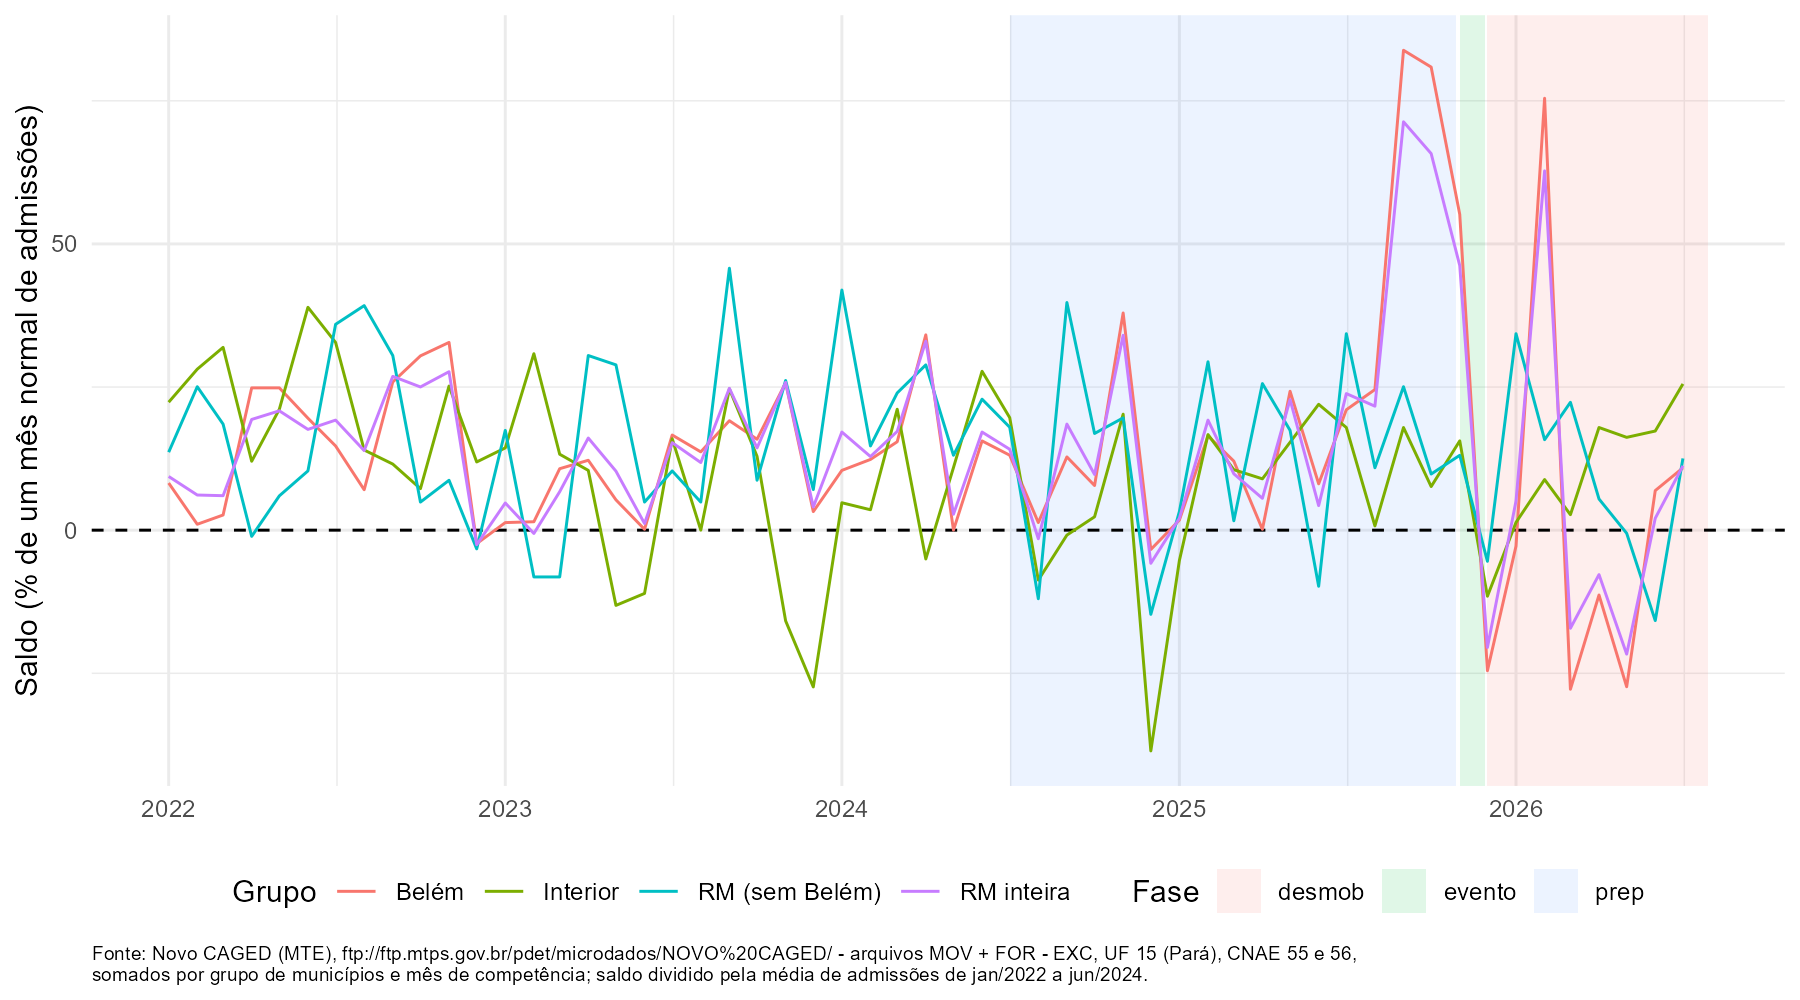
\includegraphics[width=\linewidth]{figura1_grupos.png}}%
{\fbox{\parbox{0.9\linewidth}{\centering\vspace{2cm}\afazer{Inserir figura1\_grupos.png}\vspace{2cm}}}}
\caption{Saldo normalizado por grupo, jan/2022--jul/2026, com as fases destacadas}\label{fig:grupos}
\end{figure}

\subsection{Modelo A: o padrão resiste ao ciclo macroeconômico?}

\afazer{Atualizar a Tabela~\ref{tab:modA} com o arquivo tabela2\_modeloA gerado pela nova versão do
script (controles: IBC-Br, câmbio e Selic em variação, IPCA). Na versão anterior, com o volume de
serviços do Pará como controle, Belém apresentava queda de 24,8\% (sem controles) e 28,5\% (com
controles) de um mês normal na desmobilização, ambos com $p<0{,}10$; a RM inteira, $-23{,}6\%$ e
$-25{,}9\%$; os demais municípios da RM, saldo menor no mês do evento ($-17{,}6\%$ e $-18{,}0\%$).}
O ponto central para a interpretação macroeconômica é a comparação entre os painéis sem e com
controles: se os coeficientes de fase pouco mudam, a dinâmica observada não é explicada pelo ciclo de
atividade, câmbio, juros e inflação. Os coeficientes dos próprios controles não têm interpretação
causal: variáveis nacionais que mudam lentamente podem se confundir com as fases do evento.

\begin{table}[H]
\centering\small
\caption{Modelo A: efeito por fase e grupo (MQO, erros de Newey-West)}\label{tab:modA}
\afazer{Inserir aqui a tabela tabela2\_modeloA (painel sem controles e com controles; colunas Belém,
RM sem Belém, RM inteira e Interior).}
\end{table}

\subsection{Modelo B: efeito local e transbordamento}

A Tabela~\ref{tab:modB} compara Belém e os vizinhos com o interior. Para o setor agregado, os sinais
seguem o padrão descritivo: alta na preparação (+7,6) e no evento (+26,8) e queda na desmobilização
($-8{,}1$), o que equivale a \afazer{X, Y e Z} vagas por mês em Belém. No placebo simples, esses efeitos
não se destacam dos municípios do interior; ponderados pela volatilidade de cada município, ficam entre
os três ou quatro maiores dos 26 ($p = 0{,}115$ no evento e $0{,}154$ na desmobilização), sem
significância a 10\%. Os coeficientes dos vizinhos não são estatisticamente diferentes de zero: não há
evidência de transbordamento.

\begin{table}[H]
\centering\small
\begin{threeparttable}
\caption{Modelo B: efeito local e transbordamento (interior como comparação)}\label{tab:modB}
\begin{tabularx}{\linewidth}{Lccc}
\toprule
 & Coeficiente & \multicolumn{2}{c}{p-valor do placebo}\\
\cmidrule(lr){3-4}
 & (erro agrupado) & simples & ponderado\\
\midrule
Belém $\times$ Preparação & $7{,}65$ (6,09) & 0,654 & 0,115\\
Belém $\times$ Evento & $26{,}75$ (19,52) & 0,500 & 0,115\\
Belém $\times$ Desmobilização & $-8{,}10$ (4,13) & 0,808 & 0,154\\
RM $\times$ Preparação & $1{,}81$ (8,49) & & \\
RM $\times$ Evento & $22{,}67$ (29,51) & & \\
RM $\times$ Desmobilização & $-7{,}24$ (8,77) & & \\
\midrule
Observações & 1.705 & & \\
Municípios & 31 & & \\
\bottomrule
\end{tabularx}
\begin{tablenotes}\footnotesize
\item Nota: variável dependente é o saldo normalizado do município. Efeitos fixos de município $\times$
mês do ano e de mês calendário; erros agrupados por município entre parênteses (pouco confiáveis com uma
única unidade tratada). O p-valor do placebo é a proporção dos 26 municípios (Belém e 25 do interior)
com efeito, em módulo, maior ou igual ao de Belém; no ponderado, cada efeito é dividido pelo
desvio-padrão do saldo do município em jan/2022--jun/2024.
\end{tablenotes}
\end{threeparttable}
\end{table}

\textbf{Por que os Modelos A e B diferem para os vizinhos.} No Modelo A, os vizinhos têm saldo menor no
mês do evento; no Modelo B, o coeficiente é positivo e impreciso. A diferença decorre da ponderação: no
Modelo A, os municípios são somados, e Ananindeua, o maior deles, tende a dominar a série; no Modelo B, cada
município pesa igualmente e é comparado com o interior. O resultado sugere que o deslocamento de
trabalhadores para a sede, se ocorreu, concentrou-se no maior vizinho, mas a evidência não é robusta.

\textbf{Tendências pré-evento.} \afazer{Inserir a Figura figura2\_event\_study\_para e descrever:
os coeficientes de Belém antes de julho de 2024 ficam (ou não) dentro da faixa dos municípios do
interior.}

\subsection{O efeito está na hospedagem}

A separação por setor (Tabela~\ref{tab:rob}, coluna 2) mostra que o efeito se concentra no
Alojamento: os coeficientes de Belém são de +42,3 na preparação, +104,0 no evento e $-37{,}9$ na
desmobilização, o que corresponde a \afazer{X, Y e Z} vagas por mês. A Alimentação (coluna 3) não
apresenta efeito distinguível de zero. Esse é o padrão esperado de um choque de visitantes: a
hospedagem responde primeiro e com mais força. \afazer{Inserir o p-valor do placebo para o
Alojamento (arquivo placebo\_belem, variável saldo\_norm\_55) e a comparação com as capitais.}

\subsection{Modelo C: o choque apareceu nos preços?}

\afazer{Inserir a tabela tabela4\_precos e descrever: no mês do evento, a inflação de hospedagem e de
alimentação fora do domicílio em Belém ficou (ou não) acima da nacional; comparar com o resultado de
emprego (o ajuste se deu mais por quantidade ou por preço).}

% ---------------------------------------------------------------------
\section{Robustez}

A Tabela~\ref{tab:rob} reestima o Modelo B com quatro variações. Retirar Castanhal da Região
Metropolitana (coluna 4) não altera os resultados de Belém e reduz os coeficientes dos vizinhos.
Tratar outubro a dezembro como um único bloco, para não confundir o evento com o Círio de Nazaré
(coluna 5), mantém o efeito positivo de Belém (+18,9) e a queda posterior, menor. As estrelas
reportadas usam o erro agrupado e devem ser lidas com a cautela já discutida.

\begin{table}[H]
\centering\small
\begin{threeparttable}
\caption{Modelo B: separação por setor e testes de robustez}\label{tab:rob}
\begin{tabularx}{\linewidth}{Lccccc}
\toprule
 & (1) & (2) & (3) & (4) & (5)\\
 & Principal & Alojamento & Alimentação & Sem & Out--dez\\
 & & (CNAE 55) & (CNAE 56) & Castanhal & em bloco\\
\midrule
Belém $\times$ Preparação & $7{,}65$ & $42{,}26$ & $0{,}91$ & $7{,}65$ & $4{,}94$\\
 & (6,09) & (8,76) & (7,67) & (6,10) & (6,28)\\
Belém $\times$ Evento & $26{,}75$ & $103{,}99$ & $18{,}81$ & $26{,}75$ & $18{,}94$\\
 & (19,52) & (36,91) & (22,40) & (19,54) & (6,94)\\
Belém $\times$ Desmobilização & $-8{,}10$ & $-37{,}87$ & $-5{,}39$ & $-8{,}10$ & $-6{,}57$\\
 & (4,13) & (9,18) & (6,45) & (4,13) & (4,01)\\
RM $\times$ Preparação & $1{,}81$ & $76{,}27$ & $-5{,}31$ & $-3{,}49$ & $3{,}08$\\
 & (8,49) & (44,63) & (10,41) & (7,37) & (8,38)\\
RM $\times$ Evento & $22{,}67$ & $44{,}06$ & $15{,}67$ & $11{,}26$ & $-2{,}91$\\
 & (29,51) & (153,35) & (30,03) & (31,21) & (15,61)\\
RM $\times$ Desmobilização & $-7{,}24$ & $-55{,}13$ & $-5{,}53$ & $-4{,}03$ & $-6{,}51$\\
 & (8,77) & (33,32) & (11,97) & (9,85) & (9,34)\\
\midrule
Observações & 1.705 & 1.705 & 1.705 & 1.650 & 1.705\\
\bottomrule
\end{tabularx}
\begin{tablenotes}\footnotesize
\item Nota: efeitos fixos de município $\times$ mês do ano e de mês calendário; erros agrupados por
município entre parênteses, pouco confiáveis com uma única unidade tratada. Nas colunas 2 e 3, o saldo
de cada setor é normalizado pelas admissões médias do próprio setor no período de referência. Na
coluna 5, o evento compreende outubro a dezembro de 2025 e a desmobilização começa em janeiro de 2026.
\end{tablenotes}
\end{threeparttable}
\end{table}

\textbf{Belém contra as demais capitais.} Como o interior do Pará é formado por municípios menores e
mais voláteis que Belém, o Modelo B é reestimado com outro contrafactual: as 25 demais capitais
estaduais (exceto o Rio de Janeiro), com efeitos fixos de capital $\times$ mês do ano e de mês
calendário, placebo com cada capital e controle sintético (Abadie e Gardeazabal, 2003; Abadie,
Diamond e Hainmueller, 2010), no qual Belém é comparada com uma combinação ponderada de capitais que reproduz sua trajetória antes da
preparação. \afazer{Inserir resultados de capitais\_did, capitais\_robustez e capitais\_sc\_resultado,
e as figuras capitais\_event\_study e capitais\_sc\_trajetoria.}

% ---------------------------------------------------------------------
\section{Considerações finais}

O artigo tratou a COP30 como um choque de demanda regional temporário e investigou como ele se
manifestou no mercado de trabalho formal de Alojamento e Alimentação e nos preços locais. Os
resultados apontam um efeito \textbf{local, temporário e concentrado na hospedagem}: o emprego no
Alojamento de Belém subiu nos meses que antecederam o evento e recuou depois, sem transbordamento
positivo para os demais municípios da Região Metropolitana e sem ganho líquido para a região. A
dinâmica não é explicada pelo ciclo macroeconômico nacional. Para o setor agregado, os efeitos têm a
direção esperada, mas não se distinguem da variação dos municípios do interior, o que é coerente com a
literatura de megaeventos (Hagn e Maennig, 2009; Feddersen e Maennig, 2013). \afazer{Uma frase sobre
preços (Modelo C) e uma sobre as capitais.} Para a política pública, o resultado sugere cautela com o
argumento de que grandes eventos são, por si, estratégia de geração de emprego regional.

As principais limitações são o pequeno número de municípios com emprego relevante no setor e a
existência de uma única unidade tratada, que limitam a inferência; o fato de o CAGED captar apenas o
emprego formal, em uma região de alta informalidade; e a ausência dos canais salarial e fiscal.
Extensões naturais são a análise dos salários de admissão e do tipo de contrato (temporário e
intermitente) no próprio CAGED e a incorporação do investimento público associado ao evento como
choque fiscal.

% ---------------------------------------------------------------------
\section*{Referências}
\begin{singlespace}\small
\setlength{\parindent}{0pt}\setlength{\parskip}{5pt}\raggedright

ABADIE, A.; GARDEAZABAL, J. The economic costs of conflict: a case study of the Basque Country.
\textit{American Economic Review}, v. 93, n. 1, p. 113--132, 2003.

ABADIE, A.; DIAMOND, A.; HAINMUELLER, J. Synthetic control methods for comparative case studies.
\textit{Journal of the American Statistical Association}, v. 105, n. 490, p. 493--505, 2010.

ARELLANO, M.; BOND, S. Some tests of specification for panel data. \textit{Review of Economic
Studies}, v. 58, n. 2, p. 277--297, 1991.

BAUMANN, R.; MATHESON, V. Mega-events and tourism: the case of Brazil. \textit{Contemporary Economic
Policy}, v. 36, n. 2, p. 292--301, 2018.

BLANCHARD, O. J.; KATZ, L. F. Regional evolutions. \textit{Brookings Papers on Economic Activity},
v. 1992, n. 1, p. 1--75, 1992.

BRONZINI, R.; MOCETTI, S.; MONGARDINI, M. \textit{The economic effects of big events}: evidence from
the Great Jubilee 2000 in Rome. Roma: Banca d'Italia, 2019. (Temi di discussione, n. 1208).

CONLEY, T. G.; TABER, C. R. Inference with ``difference in differences'' with a small number of
policy changes. \textit{Review of Economics and Statistics}, v. 93, n. 1, p. 113--125, 2011.

DICKEY, D. A.; FULLER, W. A. Distribution of the estimators for autoregressive time series with a unit
root. \textit{Journal of the American Statistical Association}, v. 74, n. 366, p. 427--431, 1979.

DI PIETRA, G.; PARFITT, R.; CALUZ, A. D.; GARCIA, F. Big plants in small towns: labor concentration
and land use in rural Brazil. In: ENCONTRO BRASILEIRO DE ECONOMETRIA, 48., 2026. \textit{Anais}.
[S. l.]: SBE, 2026.

FABER, B.; GAUBERT, C. Tourism and economic development: evidence from Mexico's coastline.
\textit{American Economic Review}, v. 109, n. 6, p. 2245--2293, 2019.

FEDDERSEN, A.; MAENNIG, W. Mega-events and sectoral employment: the case of the 1996 Olympic Games.
\textit{Contemporary Economic Policy}, v. 31, n. 3, p. 580--603, 2013.

FREYALDENHOVEN, S.; HANSEN, C.; SHAPIRO, J. M. Pre-event trends in the panel event-study design.
\textit{American Economic Review}, v. 109, n. 9, p. 3307--3338, 2019.

GRANGER, C. W. J.; NEWBOLD, P. Spurious regressions in econometrics. \textit{Journal of
Econometrics}, v. 2, n. 2, p. 111--120, 1974.

GREENSTONE, M.; HORNBECK, R.; MORETTI, E. Identifying agglomeration spillovers: evidence from
winners and losers of large plant openings. \textit{Journal of Political Economy}, v. 118, n. 3,
p. 536--598, 2010.

HAGN, F.; MAENNIG, W. Large sport events and unemployment: the case of the 2006 soccer World Cup in
Germany. \textit{Applied Economics}, v. 41, n. 25, p. 3295--3302, 2009.

JUDSON, R. A.; OWEN, A. L. Estimating dynamic panel data models: a guide for macroeconomists.
\textit{Economics Letters}, v. 65, n. 1, p. 9--15, 1999.

LEONI, V.; BOTO-GARCÍA, D. The effect of natural disasters on hotel demand, supply and labour
markets: evidence from the La Palma volcano eruption. \textit{Environmental and Resource Economics},
v. 86, n. 4, p. 755--780, 2023.

MENDES GARCIA, P.; MENDONÇA, H. F. Climate shocks and the unequal burden of inflation. In: ENCONTRO
BRASILEIRO DE ECONOMETRIA, 48., 2026. \textit{Anais}. [S. l.]: SBE, 2026.

MIAN, A.; SUFI, A. What explains the 2007--2009 drop in employment? \textit{Econometrica}, v. 82,
n. 6, p. 2197--2223, 2014.

MORETTI, E. Local multipliers. \textit{American Economic Review: Papers \& Proceedings}, v. 100,
n. 2, p. 373--377, 2010.

NAKAMURA, E.; STEINSSON, J. Fiscal stimulus in a monetary union: evidence from US regions.
\textit{American Economic Review}, v. 104, n. 3, p. 753--792, 2014.

NEWEY, W. K.; WEST, K. D. A simple, positive semi-definite, heteroskedasticity and autocorrelation
consistent covariance matrix. \textit{Econometrica}, v. 55, n. 3, p. 703--708, 1987.

ROODMAN, D. A note on the theme of too many instruments. \textit{Oxford Bulletin of Economics and
Statistics}, v. 71, n. 1, p. 135--158, 2009.
\end{singlespace}

\end{document}
